% informe.tex - Documentación sobre el trabajo práctico para entregar

\documentclass{article}
\usepackage[utf8]{inputenc}
\usepackage[spanish]{babel}
\usepackage{graphicx}

\begin{document}

\title{Informe Trabajo Práctico 1}
\author{Victoria Perelló (89608)\\
        \and
        Agustín Mezzina (89637)\\
	\and
        Pablo Rodríguez (93970)}
\maketitle

\section{Procesos}
La aplicación se divide en los siguientes procesos:
\begin{enumerate}
	\item Init: llena la cola de autos entrantes.
	\item Jefe de estación: recibe los autos entrantes y los asigna a empleados libres. En caso de no haber empleados libres, los despacha.
	\item Empleado: asigna autos a surtidores libres. Si no hay surtidores libres, espera a que se libere alguno. Realiza el servicio. Cobra y guarda la recaudación en la caja.
	\item Consulta caja registradora: consulta asincrónica sobre el valor de la recaudación en caja.
\end{enumerate}

\section{Comunicación entre procesos}
En el siguiente diagrama, se muestra el esquema de comunicación entre los procesos del sistema. Incluye los datos que intercambian los procesos que se comunican entre sí y los recursos a los que deben acceder de manera concurrente.
\\[1\baselineskip]
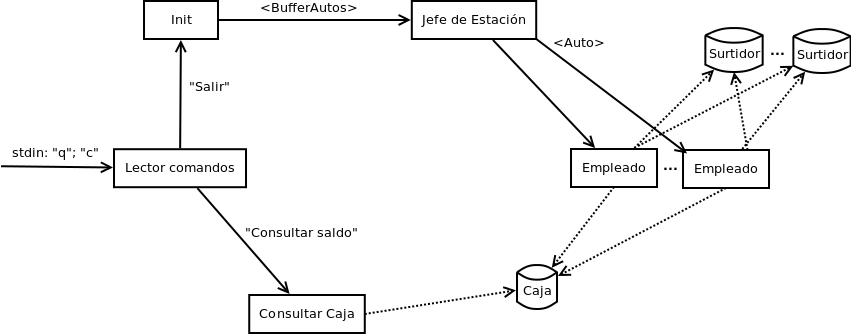
\includegraphics[width=\textwidth]{overview}

\section{Problemas conocidos de concurrencia}
\begin{enumerate}
	\item Init - Jefe de estación: Productor - Consumidor. El proceso base hace las veces de Productor, ingresando autos nuevos a un buffer compartido donde posteriormente el Jefe de Estación, en este caso Consumidor, los retira según su orden de llegada y los procesa.
	\item Jefe de estación - Empleado(s):
	\item Empleado - Empleado: Sección Crítica. Los procesos deben excluirse mutuamente al ejecutar código que acceda a los recursos Surtidores.
	\item Empleado(s) - Consultar Caja: Sección Crítica. Los procesos deben excluirse mutuamente al ejecutar código que acceda al recurso Caja.
\end{enumerate}
\section{Mecanismos de concurrencia a utilizar}
Se agregaron en el diagrama los mecanismos utilizados para lograr la comunicación y sincronización de procesos
\\[1\baselineskip]
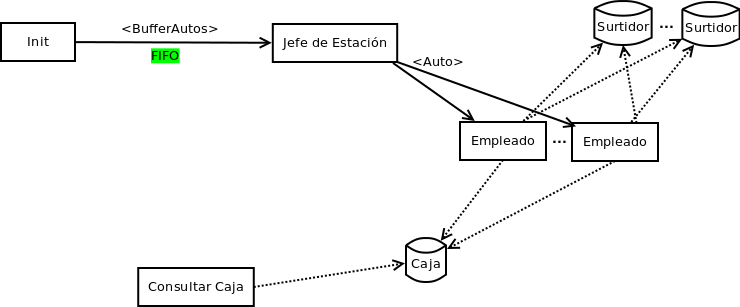
\includegraphics[width=\textwidth]{overview+mecanismos}
\begin{enumerate}
        \item Init - Jefe de estación. El buffer de autos se implementó utilizando un named pipe (o FIFO), de manera que el proceso inicial ingresa los autos al canal a medida que los va produciendo y el jefe de estación los toma en orden para procesarlos. Este mecanismo de concurrencia provee no sólo comunicación entre ambos procesos, sino que también sincronismo.
	\item Jefe de estación - Empleado(s). Se utiliza memoria compartida para ver si hay empleados libres y para asignarle un auto a ese empleado.
	*Ver lo de productor-consumidor*
	\item Empleado - Empleado: Sección Crítica. se utilizan semáforos y memoria compartida.
	\item Empleado(s) - Consultar Caja. Se utiliza un semaforo para controlar que no esté consultando o modificando la caja más de un proceso a la vez. Y se utiliza memoria compartida para guardar el valor de la caja.

\end{enumerate}
					
\end{document}
